\section{Aufgabe 9}
    \subsection{a)}
        Gegeben ist die Kurve in Polarkoordinaten:
        $$r = \frac{4}{\sqrt{12 - 8 \sin^2(\varphi)}}$$
        Wir möchten diese Kurve in kartesische Koordinaten $(x, y)$ umschreiben. Dazu verwenden wir die bekannten Beziehungen zwischen Polarkoordinaten und kartesischen Koordinaten:
        \begin{align*}
            x &= r \cos(\varphi), \\
            y &= r \sin(\varphi), \\
            r^2 &= x^2 + y^2.
        \end{align*}
        
        Da $\sin(\varphi) = \frac{y}{r} $:
        $$\Rightarrow r = \frac{4}{\sqrt{12 - 8 \left(\frac{y}{r}\right)^2}}.$$
        $$\Leftrightarrow r^2 = \frac{16}{12 - 8 \frac{y^2}{r^2}}.$$
        $$\Leftrightarrow r^2 \left(12 - 8 \frac{y^2}{r^2}\right) = 16.$$
        $$\Leftrightarrow 12 r^2 - 8 y^2 = 16.$$
        $$\text{Da } r^2 = x^2 + y^2 \Rightarrow 12(x^2 + y^2) - 8 y^2 = 16.$$
        $$\Rightarrow 12x^2 + 4y^2 = 16.$$
        $$ \Rightarrow \frac{3x^2}{4} + \frac{y^2}{4} = 1.$$
        Dies ist die Gleichung einer Ellipse in kartesischen Koordinaten:
        $$\Rightarrow \frac{x^2}{\frac{4}{3}} + \frac{y^2}{4} = 1.$$

        Die Kurve in kartesischen Koordinaten ist also eine Ellipse mit Halbachsen \(\sqrt{\frac{4}{3}}\) entlang der \(x\)-Achse und \(2\) entlang der \(y\)-Achse.
    \subsection{b)}
        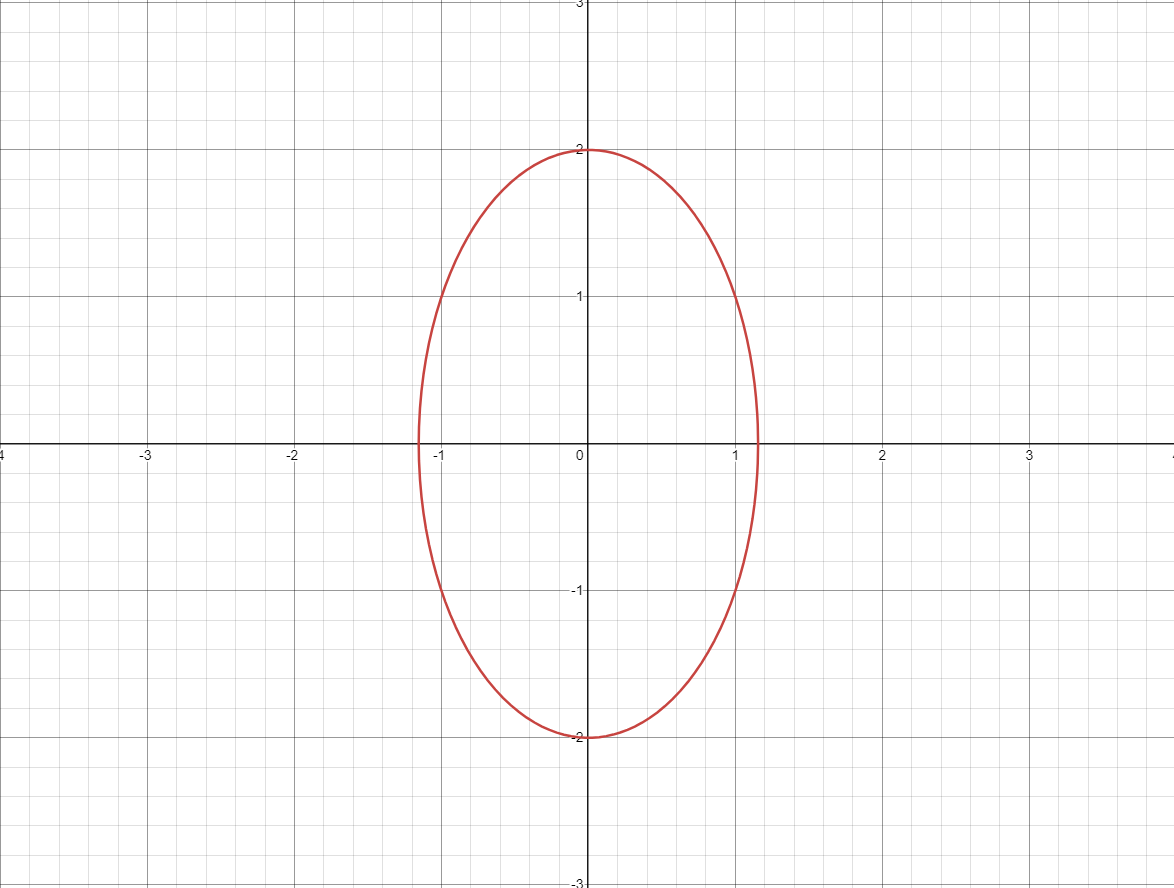
\includegraphics[width=\textwidth]{Aufgaben/09/9b).png}